\par\noindent\begin{minipage}{\linewidth}
    \centering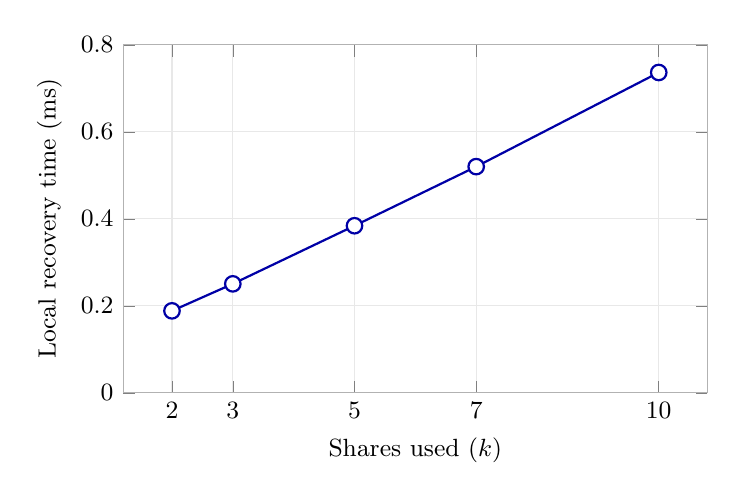
\begin{tikzpicture}
        \begin{axis}[width=9cm,height=6cm,grid=major,major grid style={gray!18},axis line style={gray!60},tick label style={font=\small},label style={font=\small},scaled ticks=false,xlabel={Shares used ($k$)},ylabel={Local recovery time (ms)},xtick={2,3,5,7,10},ymin=0,ymax=0.8]
            \addplot[color=blue!65!black,mark=*,mark size=2.8pt,mark options={fill=white},thick] coordinates {(2,0.188436) (3,0.250553334) (5,0.384199667) (7,0.520116083) (10,0.736622708)};
        \end{axis}
    \end{tikzpicture}
    \par\smallskip{\small 그림 5. Committee n=10에서 share k 증가에 따른 Master Key 복구 시간.}\par\medskip
    {\small\setlength{\tabcolsep}{7pt}
        \begin{tabular}{@{}rr@{}}\toprule
            \textbf{share k} & \textbf{복구 시간 (ms)} \\
            \midrule
            2                & 0.188               \\
            3                & 0.251               \\
            5                & 0.384               \\
            7                & 0.520               \\
            10               & 0.737               \\
            \bottomrule
        \end{tabular}}
\end{minipage}\par\medskip
